\documentclass[a4paper,10pt]{article}
%\usepackage[latin1]{inputenc}
\usepackage{amsfonts}
\usepackage{amssymb}
\usepackage{amsthm}
\usepackage{amsmath}
\usepackage{caption}
\usepackage{booktabs}
\usepackage[bahasai]{babel}
\usepackage[hidelinks]{hyperref}
%\usepackage[labelsep=period,format=hang,font=small]{caption}
\usepackage{caption}
\usepackage{fontenc}
\usepackage{graphicx}
\usepackage{lipsum}
\usepackage{abstract}
\usepackage{times}
\usepackage{indentfirst}
\usepackage{url}
\usepackage{titlesec}
\usepackage{multicol}
\usepackage{multirow}
\usepackage{titling}
\usepackage{tabularx}
\usepackage{microtype}
\usepackage{tikz}
\usepackage{subfig}
\usepackage{enumitem}
\usepackage{rotating}
\usepackage{makecell}
\usepackage{colortbl}
\setlength{\droptitle}{-1.5cm}
\urlstyle{rm}
\renewcommand{\baselinestretch}{1}

\setlength{\footskip}{40pt}

\usepackage[top=19mm,bottom=43mm,left=14.32mm,right=14.32mm]{geometry}
\setlength{\tabcolsep}{4.22mm}
\renewcommand\thesection{\Roman{section}}
\renewcommand\thesubsection{\Alph{subsection}}
\renewcommand\thesubsubsection{\arabic{subsubsection})}
\renewcommand\thetable{\Roman{table}}
%\newcommand{\SSS}{\renewcommand{\baselinestretch}{1.5}\tiny \normalsize }
%\newcommand{\SDS}{\renewcommand{\baselinestretch}{1}\tiny \normalsize }

\titleformat{\section}[block]{\normalsize\filcenter\scshape\Roman{section}.}{}{0.5em}{}
\titleformat{name=\section,numberless}[block]{\normalsize\filcenter\scshape}{}{0em}{}
\titleformat{\subsection}[block]{\normalsize\itshape\Alph{subsection}.}{}{0.5em}{}
\titleformat{\subsubsection}[runin]{\normalsize\itshape}{\thesubsubsection}{0.5em}{}[:]
\titlespacing{\section}{0em}{0.25em}{0.5em}
\titlespacing{\subsection}{0em}{0.25em}{0.5em}
\titlespacing{\subsubsection}{1em}{0.25em}{0.5em}
\newenvironment{body}{\begin{multicols}{2}}{\end{multicols}}
\setlength{\parskip}{0mm}

\addto\captionsbahasai{
	\renewcommand{\abstractname}{Intisari}
	\renewcommand{\bibname}{Referensi}
	\renewcommand{\refname}{Referensi}
	\renewcommand{\tablename}{\scshape{TABEL}}
}

\let\oldthebibliography\thebibliography
\let\endoldthebibliography\endthebibliography
\renewenvironment{thebibliography}[1]{
	\begin{oldthebibliography}{#1}
		\setlength{\itemsep}{0em}
		\setlength{\parskip}{0em}
	}
	{
	\end{oldthebibliography}
}

\captionsetup[table]{format=plain,labelsep=newline,font=footnotesize,textfont=sc,justification=centering}
\captionsetup[figure]{labelsep=period,format=hang,font=footnotesize,justification=justified}

\makeatletter
\renewenvironment{table}
{\def\@captype{table}%
	\captionsetup{format=plain,labelsep=newline,font=footnotesize,textfont=sc,justification=centering}%
	\fontsize{8}{8}\selectfont
}
{}

\renewenvironment{figure}
{\def\@captype{figure}%
	\captionsetup{labelsep=period,format=hang,font=footnotesize,justification=justified}
}
{}

\makeatother

\newcommand*\annotatedFigureBoxCustom[8]{\draw[#5,thick,rounded corners] (#1) rectangle (#2);\node at (#4) [fill=#6,thick,shape=circle,draw=#7,inner sep=2pt,font=\sffamily,text=#8] {\textbf{#3}};}
%\annotatedFigureBox{bottom-left}{top-right}{label}{label-position}
\newcommand*\annotatedFigureBox[4]{\annotatedFigureBoxCustom{#1}{#2}{#3}{#4}{white}{white}{black}{black}}
\newcommand*\annotatedFigureText[4]{\node[draw=none, anchor=south west, text=#2, inner sep=0, text width=#3\linewidth,font=\sffamily] at (#1){#4};}
\newenvironment {annotatedFigure}[1]{\begin{tikzpicture}
	\node[anchor=south west,inner sep=0] (image) at (0,0) { #1};\begin{scope}[x={(image.south east)},y={(image.north west)}]}{\end{scope}\end{tikzpicture}}

\usetikzlibrary{shapes.geometric, arrows, positioning,datavisualization,patterns,decorations.markings,calc,intersections}
\tikzstyle{startstop} = [rectangle, rounded corners, minimum width=3cm, minimum height=1cm,text centered, draw=black]
\tikzstyle{io} = [trapezium, trapezium left angle=70, trapezium right angle=110, minimum width=3cm, minimum height=1cm, text centered, draw=black]
\tikzstyle{process} = [rectangle, minimum width=3cm, text width=5.5cm, minimum height=1cm, text centered, draw=black]
\tikzstyle{decision} = [diamond, minimum width=3cm, minimum height=1cm, text centered, draw=black]
\tikzstyle{arrow} = [thick,->,>=stealth]

%\renewenvironment{abstract}
%{\list{}{%
%	}%
%	\item[\noindent\textbf{\abstractname ---}]\relax}
%{\endlist}

\title{\fontsize{24}{28}\selectfont Perancangan Kontroler Lingkungan Termal \textit{Climate Chamber} Berbasis Jaringan Saraf Tiruan}
\author{\fontsize{11}{11}\selectfont Ridhan Fadhilah$^1$, Faridah$^2$, Agus Arif$^3$}
\date{}

\begin{document}
	\setlength{\abovedisplayskip}{1pt}
	\setlength{\belowdisplayskip}{1pt}	
	
	\maketitle
	
	\vspace{-1.5cm}
	
	{\centering
		{\itshape\fontsize{10}{10}\selectfont
			$^{1,2,3}$Departemen Teknik Nuklir dan Teknik Fisika FT UGM\\
			Jln. Grafika 2 Yogyakarta 55281 INDONESIA\\
		}
		{\fontsize{9}{9}\normalfont\selectfont
			$^1$ridhan.fadhilah@mail.ugm.ac.id\\
			$^2$faridah@ugm.ac.id\\
			$^3$agusarif@ugm.ac.id\\
		}
	}
	
	\vspace{0.3cm}
	
	{\setlength{\parindent}{0cm}\bfseries
		Intisari--- Penelitian-penelitan kenyamanan termal membutuhkan kondisi lingkungan termal pada \textit{climate chamber} (sebagai ruang uji eksperimental) untuk dapat dikondisikan secara otomatis sesuai dengan skema pengujian penelitian. \textit{Climate chamber} dapat terwujud jika kondisi iklim di dalamnya dapat dikendalikan sesuai dengan kebutuhan skenario penelitian. Oleh karena itu, dibutuhkan suatu sistem kontrol yang mampu mengendalikan lingkungan termal pada \textit{climate chamber}.
		
		\qquad Penelitian ini menggunakan sampel data sebanyak 24.000 yang didapatkan dari simulasi IES-VE. Dengan menggunakan data tersebut, dibangun kontroler berbasis jaringan saraf tiruan (JST) untuk mengendalikan suhu ruang (T$_{db}$) dan kelembapan relatif (RH) pada \textit{climate chamber}. Kontroler dibangun dari model JST dengan menggunakan prinsip model invers dari model \textit{plant} berdasarkan data simulasi IES-VE. Kontroler dirancang dengan memvariasikan pembagian data pelatihan, fungsi aktivasi, serta banyak neuron pada \textit{hidden layer}. Model dipilih berdasarkan nilai \textit{mean squared errror} terkecil dari hasil variasi model. Simulasi kontrol dilakukan dengan skenario pemanasan dengan laju 0,625$^\circ$C. Kinerja hasil simulasi ditinjau melalui nilai \textit{steady-state error}.
		
		\qquad Kontroler dibangun dengan menggunakan MATLAB dan disimulasikan dengan menggunakan Simulink. Model JST Kontroler dibangun dengan pembagian data 80\% data latih, 10\% data validasi, dan 10\% data uji. Model JST Kontroler menggunakan fungsi aktivasi \textit{hyperbolic tangent} dengan algoritma pembelajaran Levenberg-Marquardt. Model JST Kontroler memiliki arsitektur jaringan dengan 1 lapisan tersembunyi (\textit{hidden layer}) berisi 35 neuron. Hasil perancangan mampu mengendalikan lingkungan termal \textit{climate chamber} dengan nilai \textit{steady-state error} sebesar 0,18$^\circ$C untuk suhu ruang dan sebesar 0,04\% untuk kelembapan relatif.\\
		
		Kata kunci--- Lingkungan Termal, Kontroler, Jaringan Saraf Tiruan, Ruang Iklim.
	}
	
	\vspace{0.3cm}
	
	{\setlength{\parindent}{0cm}\bfseries
		Abstract--- Thermal comfort studies require the thermal environment conditions in the climate chamber (as a thermal test room) to be automatically conditioned according to the research test scheme. Climate chamber can be realized if the climatic conditions in it can be controlled according to the needs of the research scenario. Therefore, we need a control system capable of controlling the thermal environment in the climate chamber.
		
		\qquad This study uses a sample of 24,000 data obtained from the IES-VE simulation. By using this data, a controller based on an artificial neural network (ANN) was built to control air temperature (T$_{db}$) and relative humidity (RH) in the climate chamber. The Controller is designed from ANN model using the principle of plant inverse model based on IES-VE simulation data. Controller was designed by varying the distribution of training data, activation functions, and many neurons in the hidden layer. The model is selected based on the smallest mean squared error from the variation in the model. The control simulation is carried out with a heating scenario with a rate of 0.625 der C. The performance of the simulation results is reviewed through the steady-state error value.
		
		\qquad Controller was built using MATLAB and simulated using Simulink. ANN Controller was created by split the data into 80\% training data, 10\% validation data, and 10\% testing data. ANN controller uses the hyperbolic tangent activation function with the Levenberg-Marquardt learning algorithm. ANN Controller has a network architecture with one hidden layer containing 35 neurons. The results of the author's design able to control the thermal environment of the climate chamber with a steady-state error value 0.18$^\circ$C for room temperature and 0.04\% for relative humidity.\\
		
		Keywords--- Thermal Environment, Controller, Artificial Neural Network, Climate Chamber.
	}

	\vspace{2cm}
	
	\begin{body}
		\section{Pendahuluan}
		
		\subsection{Latar Belakang}\label{latar belakang}
		
		\textit{Climate chamber} merupakan suatu ruangan tertutup yang digunakan untuk menguji efek dari kondisi lingkungan yang ditentukan pada objek biologis, produk industri, bahan, dan/atau perangkat elektronik. Pada penulisan ini, \textit{climate chamber} yang dimaksud berfokus pada objek biologis mengenai penelitian kenyamanan termal. Dalam melakukan penelitian kenyamanan termal, peneliti tersebut membutuhkan suatu \textit{climate chamber} untuk dapat melakukan pengujian. Kondisi lingkungan termal di dalam \textit{climate chamber} dapat berubah sesuai dengan skema pengujian. Terdapat 6 faktor lingkungan termal yang mempengaruhi kenyamanan termal. Faktor lingkungan termal tersebut meliputi tingkat metabolisme tubuh, insulasi pakaian, suhu udara, suhu radian, kecepatan udara dan kelembapan \cite{ASHRAE55}.
		
		\begin{figure}
			\centering
			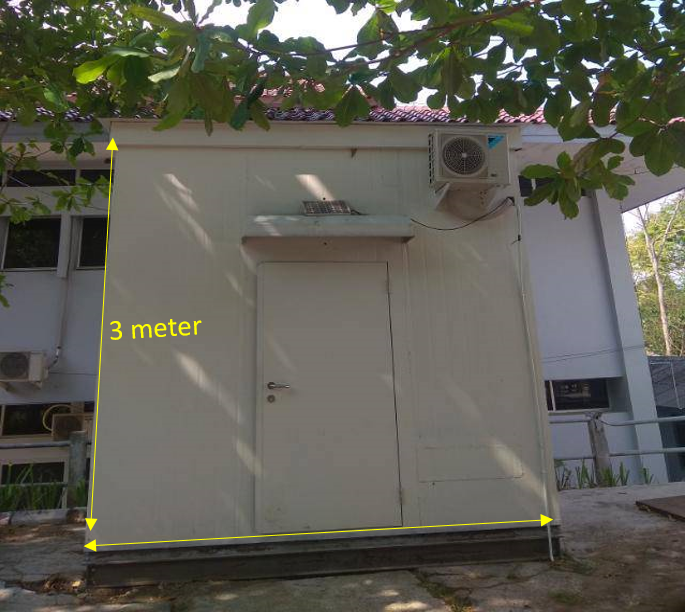
\includegraphics[width=0.4\textwidth]{figures/climatechamber}
			\caption{\textit{Climate chamber} DTNTF FT-UGM}
			\label{fig:1:climatechamber}
		\end{figure}
		
		\textit{Climate chamber} dapat terwujud jika kondisi iklim di dalamnya dapat dikendalikan sesuai dengan kebutuhan penelitian. Oleh karena itu, dibutuhkan suatu sistem kontrol yang mampu mengendalikan lingkungan termal pada \textit{climate chamber} dengan meninjau nilai \textit{steady-state error} suhu ruang dan kelembapan relatif. \textit{Climate chamber} memiliki banyak nilai masukan dan keluaran atau dikatakan sebagai sistem MIMO (\textit{multiple input multiple output}). Untuk dapat mengendalikan sistem MIMO, diperlukan sistem kontrol cerdas (\textit{intelligent control system}). Salah satu sistem kontrol cerdas yang dapat digunakan untuk sistem MIMO ini yaitu pengendali dengan menggunakan jaringan saraf tiruan (\textit{neural network controller}).\\
		
		\subsection{Perumusan Masalah}
		Perumusan masalah pada penelitian ini yaitu bagaimana merancang kontroler lingkungan termal berbasis jaringan saraf tiruan untuk dapat mencapai kondisi ajeg sesuai dengan skenario penggunaan \textit{climate chamber} DTNTF FT-UGM.\\
		
		\subsection{Tujuan}
		Penelitian ini bertujuan untuk membangun model kontroler berbasis jaringan saraf tiruan dengan meninjau nilai \textit{steady-state error} untuk mengendalikan lingkungan termal pada \textit{climate chamber} DTNTF FT-UGM.\\
		
		\subsection{Batasan Masalah}
		Berikut batasan masalah dalam penelitian ini:
		\begin{enumerate}
			\item Data yang digunakan merupakan data simulasi IES-VE.
			\item Model \textit{plant} dibangun dengan menggunakan model jaringan saraf tiruan.
			\item Kinerja kontroler hanya ditinjau melalui nilai \textit{steady-state error} karena secara fisis respon transien termal pada bangunan berlangsung cukup lama.
			\item \textit{Climate chamber} dituntut untuk mampu menjaga kondisi lingkungan termal pada nilai tertentu dengan galat suhu kurang dari $\pm$1$^{\circ}$C dan galat kelembapan relatif kurang dari $\pm$10\%.
			%\item Penelitian hanya berfokus pada bagian \textit{controller} dari keseluruhan sistem pengendalian. %Penelitian ini tidak membahas sensor, aktuator atau sistem komunikasi data.
			%\item Penelitian ini tidak membahas karakterisasi sistem lingkungan termal secara mendalam dan lebih berfokus pada rancangan kontroler.
		\end{enumerate}
		
		\vspace{2mm}
		
		\subsection{Manfaat}
		Berikut manfaat dari penelitian ini:
		\begin{enumerate}
			\item Penelitian ini diharapkan mampu mengembangkan ilmu pengetahuan dan aplikasinya di bidang fisika bangunan, sistem kontrol dan kecerdasan buatan.
			\item Penelitian ini diharapkan mampu menjadi referensi bagi praktisi kecerdasan buatan atau praktisi dalam pengembangan kenyamanan termal suatu bangunan.
			\item Penelitian ini diharapkan mampu memajukan perkembangan teknologi sistem bangunan di Indonesia.
		\end{enumerate}
		
		\vspace{2mm}
		
		\section{Metodologi Penelitian}
		
		\subsection{Alat dan Bahan}
		Alat dan bahan disajikan pada Tabel \ref{tbl:4:alatbahan} dan Tabel \ref{tbl:4:speklaptop}.
		
		\begin{table}
			\centering
			\caption{Daftar alat dan bahan}
			\label{tbl:4:alatbahan}
			\fontsize{8}{8}\selectfont
			\begin{tabularx}{\linewidth}{clX}\toprule
				No. & Nama alat/bahan & Fungsi \\
				\toprule
				1 & ASUS N550JX & Perangkat komputer \\ \midrule
				2 & \textit{Climate Chamber} & Objek penelitian \\ \midrule
				3 & IES-VE 2019 & Perangkat lunak untuk pengambilan data lingkungan termal \textit{climate chamber} dan variasi gangguan \\ \midrule
				4 & MS Excel 365 & Perangkat lunak pengolahan data tabular \\ \midrule
				5 & MATLAB R2018a & Perangkat lunak pemrograman dalam merancang jaringan saraf tiruan untuk kontroler. \\ \midrule
				6 & SIMULINK & Perangkat lunak untuk mewujudkan simulasi sistem kontrol. \\ \bottomrule
			\end{tabularx}
		\end{table}
		
		\begin{table}
			\centering
			\caption{Spesifikasi laptop ASUS N550JX}
			\label{tbl:4:speklaptop}
			\fontsize{8}{8}\selectfont
			\begin{tabularx}{\linewidth}{clX}\toprule
				No. & Komponen & Spesifikasi \\ \toprule
				1 & \textit{Processor} & Intel Core i7-4720HQ CPU @ 2.60GHz x 8 \\ \midrule
				2 & \textit{Graphics} & Intel Haswell Mobile \\ \midrule
				3 & RAM & 8 GB \\ \midrule
				4 & Tipe sistem operasi & 64-bit \\ \midrule
				5 & Sistem operasi & Windows 10 Home Single Language \\ \bottomrule
			\end{tabularx}
		\end{table}
		
		\subsection{Penentuan Tuntutan Rancangan}
		
		Tuntutan rancangan Tugas Akhir ini yaitu kontroler mampu mengendalikan \textit{plant} pada skenario penggunaan \textit{climate chamber} dengan galat suhu kurang dari $\pm$1$^\circ$C dan galat kelembapan relatif kurang dari $\pm$10\%.\\
		
		\subsection{Pengambilan Data Simulasi IES-VE}\label{subsec:lang_bench}
		
		Pada penelitian ini, digunakan model IES-VE untuk melakukan proses simulasi lingkungan termal. Bersamaan dengan penelitian Hartanto \cite{skripsiTanto}, data bersumber dari model yang telah dibuat pada penelitian sebelumnya berjudul "Karakterisasi Lingkungan Termal Chamber Iklim Menggunakan Metode Simulasi CFD dengan Perangkat Lunak IES-VE" yang diteliti oleh Kurniawan \cite{skripsiIchfan}.  Data tersebut merupakan hasil simulasi pada \textit{software} IES-VE dengan menerapkan beberapa variasi kondisi lingkungan pada model \textit{climate chamber}. Variasi tersebut yaitu kondisi batas lingkungan (radiasi matahari dan suhu bola kering luar/\textit{outdoor dry bulb temperature}), kondisi AC, dan kondisi \textit{heater}. Variasi kondisi batas lingkungan tersebut diwujudkan dalam pembagian 4 musim dalam 1 tahun, yakni bulan Maret, Juni, September dan Desember. Keluaran dari model IES-VE berupa nilai suhu ruang (\textit{air temperature}) \textit{chamber} dan kelembapan relatif (RH) \textit{chamber}. Dari model tersebut didapatkan nilai MAE perhitungan selisih variabel lingkungan termal hasil simulasi dan pengukuran lapangan sebesar 0,8 $\pm$ 0,7$^{\circ}$C untuk suhu udara ruang dan 2,5 $\pm$ 3,8\% untuk kelembaban relatif \cite{skripsiIchfan}. Data yang sudah terkumpul disajikan dalam bentuk tabular dan diolah dengan menggunakan komputer.\\
		
		\subsubsection{Kondisi \textit{Climate Chamber}}
		
		Climate chamber memiliki ukuran panjang $\times$ lebar $\times$ tinggi = 3 m $\times$ 2 m $\times$ 3 m. Komponen-komponen di dalam \textit{climate chamber} terdiri dari meja, kursi, \textit{blower}, penghuni, lampu, \textit{heater}, dan AC. Posisi setiap komponen di dalam \textit{climate chamber} digambarakan pada Gambar \ref{fig:4:KondisiChamber}.
		
		\begin{figure}
			\centering
			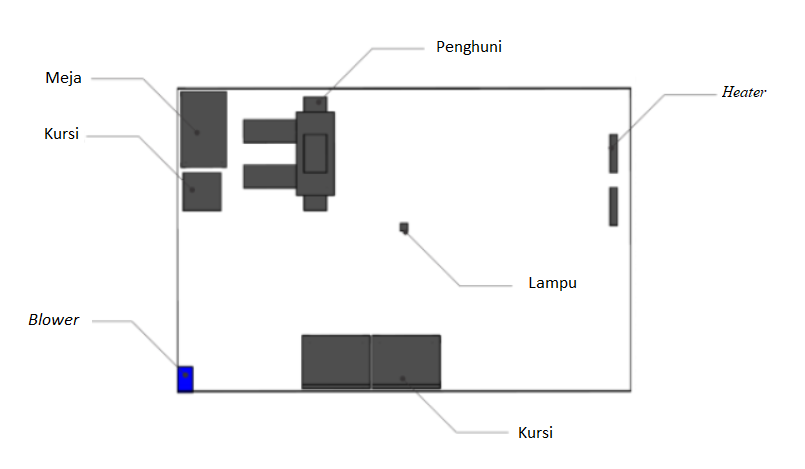
\includegraphics[width=0.4\textwidth]{figures/KondisiChamber}
			\caption{Posisi Komponen-Komponen di dalam \textit{Climate Chamber}}
			\label{fig:4:KondisiChamber}
		\end{figure}
		\vspace{2mm}
		
		Perangkat AC yang berada di dalam \textit{Climate Chamber} DTNTF FT-UGM memiliki daya sebesar 2800W (1 PK). Perangkat AC mampu mengkondisikan lingkungan melalui aliran udara yang keluar. Oleh karena itu, Perangkat AC sangatlah berpengaruh terhadap kondisi lingkungan termal di dalam ruangan. Penampakan wujud perangkat AC dapat dilihat pada Gambar \ref{fig:4:AC}\\
		
		\begin{figure}
			\centering
			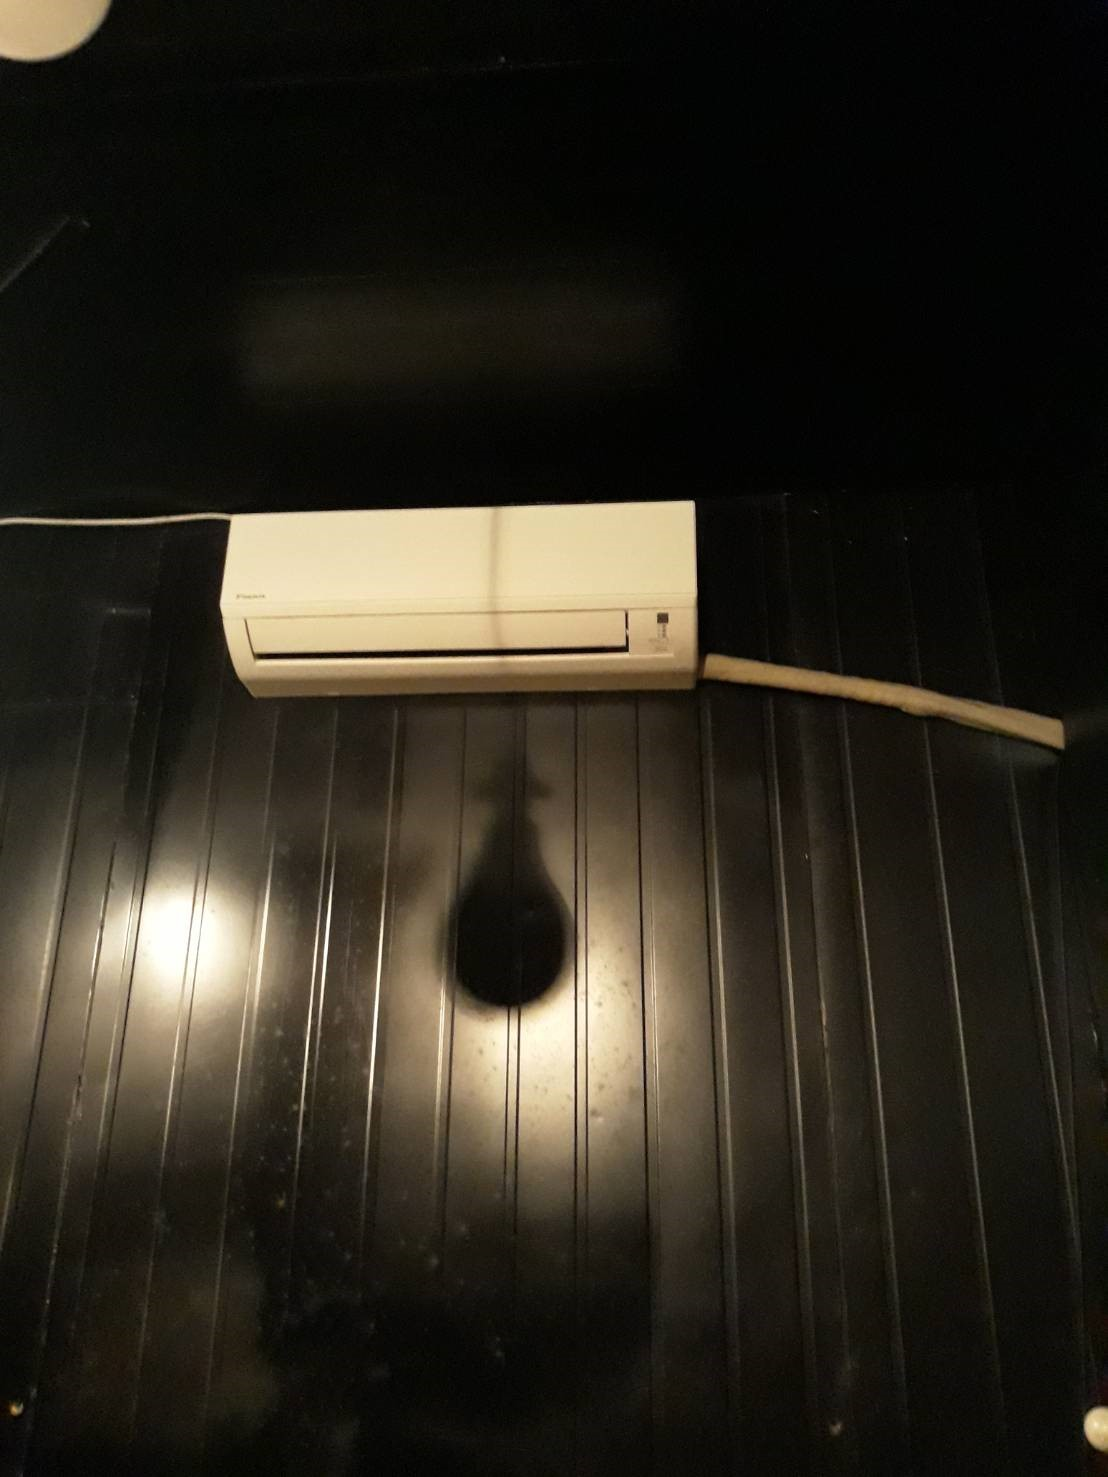
\includegraphics[width=0.25\textwidth]{figures/AC}
			\caption{Perangkat AC}
			\label{fig:4:AC}
		\end{figure}
		\vspace{1em}
		
		Perangkat pemanas (\textit{heater}) yang berada di dalam \textit{climate chamber} memiliki daya sebesar 900W. Terdapat dua buah perangkat pemanas di dalam \textit{climate chamber}. Semakin banyak perangkat pemanas yang aktif maka suhu ruang akan menjadi semakin meningkat. Kenaikan rerata suhu ruang yaitu sebesar $\pm1,9^\circ$C untuk setiap perangkat pemanas. Penampakan wujud \textit{heater} dapat dilihat pada Gambar \ref{fig:4:Heater}.\\
		
		\begin{figure}
			\centering
			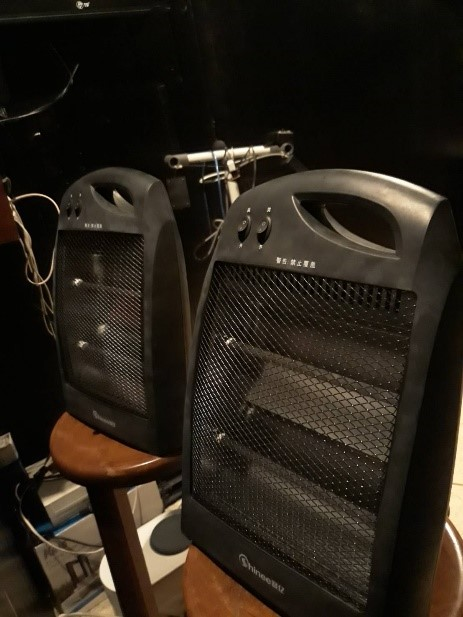
\includegraphics[width=0.15\textwidth]{figures/Heater}
			\caption{Perangkat Heater}
			\label{fig:4:Heater}
		\end{figure}
		\vspace{2mm}
		
		Selain faktor di dalam \textit{climate chamber}, faktor dari luar ruangan pun secara tidak langsung mempengaruhi kondisi lingkungan termal \textit{climate chamber}, di antaranya adalah suhu lingkungan (\textit{dry bulb temperature}) dan intensitas radiasi matahari. Posisi harian matahari mempengaruhi perubahan nilai suhu lingkungan dan intensitas radiasi matahari. Pada siang hari (posisi \textit{altitude} matahari ketika berada tepat di atas \textit{climate chamber}) memberikan paparan radiasi matahari yang mengenai selubung bangunan. Hal ini menyebabkan kenaikan suhu di dalam \textit{climate chamber}.\\
		
		\subsubsection{Rancangan Skenario Pengambilan Data}
		Rancangan skenario pada \textit{climate chamber} menghasilkan kombinasi antara perangkat AC dan jumlah \textit{heater} dalam kondisi ON. Peangkat AC dikondisikan untuk menyala dari pukul 08:00 sampai dengan pukul 17:00 WIB bervariasi dengan rentang nilai 16$^\circ$C - 30$^\circ$C dengan lompatan 1$^\circ$C. Jumlah \textit{heater} dalam kondisi ON terbagi menjadi 3 kondisi, yaitu keduanya tidak menyala (berkode 0), salah satu menyala (berkode 1), dan keduanya menyala (berkode 2). Kombinasi tersebut menghasilkan 25 variasi skenario. Untuk variasi suhu lingkungan dan intensitas radiasi matahari digunakan 4 titik ekstrim bumi terhadap matahari yaitu pada tanggal 21 Maret, 21 Juni, 23 September dan 22 Desember. Kemudian dilakukan simulasi pada setiap titik tersebut dengan kombinasi pada Gambar \ref{fig:4:SkenarioData}. Dengan demikian, total skenario yang dihasilkan dari kombinasi tersebut berjumlah 100 skenario.\\
		
		\begin{figure}
			\centering
			
\includegraphics[width=0.3\textwidth]{figures/SkenarioData}
			\caption{Skenario Pengambilan Data}
			\label{fig:4:SkenarioData}
		\end{figure}
		\vspace{2mm}
		
		\subsection{Model JST Plant}\label{subsec:4:err}
		
		Model \textit{plant} pada penelitian ini menggunakan model JST yang telah dibangun oleh Hartanto pada \cite{skripsiTanto}. Arsitektur Model Plant JST digambarkan pada Gambar \ref{fig:4:NNPlantModelDesign}. Model plant yang digunakan memiliki nilai MAE perhitungan antara target dan prediksi sebesar 0,59$^{\circ}$C untuk suhu ruang dan 5,44\% untuk kelembapan relatif. Akurasi JST sebesar 96,23\% untuk suhu ruang dan 68,90\% untuk kelembapan relatif. Keseluruhan nilai \textit{hyperparameter} model JST yang dirangkum pada Tabel \ref{tbl:5:NNPlantTanto}.\\
		
		\begin{figure}
			\centering
			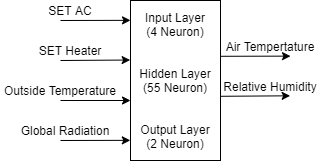
\includegraphics[width=0.3\textwidth]{figures/NNPlantModelDesign}
			\caption{Arsitektur Model Plant JST}
			\label{fig:4:NNPlantModelDesign}
		\end{figure}
	
		\begin{table}
			\caption{Tabel Rancangan Model Plant JST\cite{skripsiTanto}}
			\label{tbl:5:NNPlantTanto}
			\centering
			% use packages: array
			\begin{tabularx}{\linewidth}{ll}\toprule
				\textbf{Nama Hyperparameter} & \textbf{Nilai Hyperparameter} \\ \toprule
				Arsitektur & Feedforward Neural Network \\ \midrule
				Pembagian Data & 50\% 25\% 25\% \\ \midrule 
				Jumlah Layar Tersembunyi & 1 \\ \midrule
				Jumlah Neuron pada Layar & [55] \\ \midrule
				Fungsi Aktivasi Layar & Hyperbolic Tangent \\ \midrule
				Algoritma Pembelajaran & Levenberg-Marquardt \\ \midrule
				Mean Absolute Error (MAE) & Tdb: 0,59$^\circ$C ; RH: 5,44\% \\ \midrule
				Mean Squared Error (MSE) & Tdb: 0,75$^\circ$C ; RH: 52,33\% \\ \midrule
				Koefisien Korelasi (R) & Tdb: 96,23\% ; RH: 68,90\% \\ \bottomrule
			\end{tabularx}
		\end{table}
		
		\subsection{Perancangan Kontroler JST}
		
		Dalam melakukan pemodelan kontrol, pertama-tama didefinisikan terlebih dahulu pasangan data masukan dan keluaran dari sistem kendali. Pasangan data masukan dan keluaran tersebut didapatkan dengan memperhatikan diagram blok sistem pengendalian yang ditunjukkan pada Gambar \ref{fig:4:ConstrolSystemBlockDiagram}. Nilai pasangan masukan dan keluaran kontrol ditunjukkan pada Gambar \ref{fig:4:NNControlIO}.\\
		
		\begin{figure}
			\centering
			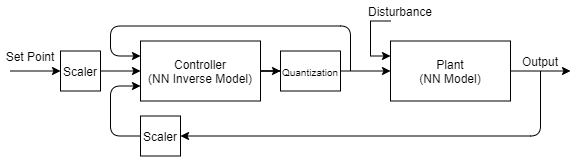
\includegraphics[width=0.5\textwidth]{figures/ControlDesignDiagramII}
			\caption{Diagram blok sistem kontrol berbasis JST\cite{paper42Paisan}}
			\label{fig:4:ConstrolSystemBlockDiagram}
		\end{figure}
	\vspace{1em}
		
		\begin{figure}
			\centering
			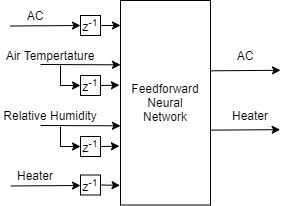
\includegraphics[width=0.25\textwidth]{figures/NNControllerIO}
			\caption{Pasangan masukan dan keluaran model JST kontroler}
			\label{fig:4:NNControlIO}
		\end{figure}
	
		Kontroler dibangun dari model JST dengan menggunakan prinsip model invers dari model \textit{plant}. Perancangan JST untuk kontroler menggunakan \textit{delay} umpan balik AC, \textit{delay} umpan balik \textit{heater}, output \textit{plant} dan \textit{delay} output \textit{plant} sebagai sebagai masukan untuk pelatihan JST. Kemudian, pasangan data AC dan \textit{heater} digunakan sebagai pasangan data keluaran (data target) untuk pelatihan JST. Arsitektur JST kontroler dibangun dengan menggunakan \textit{feedforward neural network} atau biasa disebut juga sebagai \textit{multilayer perceptron} (MLP). Model JST akan dilatih menggunakan data hasil simulai IES-VE yang telah digunakan pula dalam pemodelan \textit{plant} oleh Hartanto \cite{skripsiTanto}. Pada proses pelatihan JST, dilakukan penskalaan terhadap semua input JST menggunakan metode \textit{Min Max Scaling} kecuali variabel \textit{delay} umpan masuk AC dan \textit{heater}. Penskalaan bertujuan untuk meningkatkan kinerja JST menjadi optimal dengan menyamakan rentang nilai dan besar satuan dari setiap variabel (berupa rentang nilai dari 0 hingga 1).
		
		Perancangan model JST kontroler dilakukan dengan membandingkan variasi pembagian data latih, data validasi, dan data uji. Kemudian akan divariasikan pula fungsi aktivasi dan jumlah neuron untuk memperoleh model JST yang optimal. Evaluasi kinerja model JST kontroler menggunakan perbandingan nilai MSE pada setiap rancangan. Rancangan model JST dengan nilai MSE terkecil akan digunakan sebagai model kontroler.\\
		
		\section{Hasil dan Pembahasan}
		
		\subsection{Pengambilan Data Simulasi IES-VE}
		
		Pada Gambar \ref{fig:4:HasilSimulasiIESVE} ditunjukkan salah satu hasil simulasi untuk skenario AC 26$^\circ$C dan \textit{heater} ON 2 buah dengan variabel gangguan yang digambarkan pada Gambar \ref{fig:4:LoadSimulasiIESVE}. Grafik yang ditampilkan terdiri dari 4 parameter yaitu suhu lingkungan (T$_o$), intensitas radiasi matahari (RD), suhu ruang (T$_{db}$), dan kelembapan relatif (RH). Skenario ini dilakukan selama 24 jam dengan selang waktu pengambilan data selama 6 menit dimulai dari pukul 00:03 hingga 23:57 WIB. Selang waktu tersebut adalah waktu tersingkat yang dapat dilakukan pada software IES-VE 2019. Respon waktu suhu ruang terhadap aktivasi AC tidak diperhitungkan dikarenakan secara fisis, respons transien termal pada bangunan berlangsung cukup lama, sehingga hanya berfokus untuk meninjau nilai \textit{steady-state error}.\\
		
		\begin{figure}
			\centering
			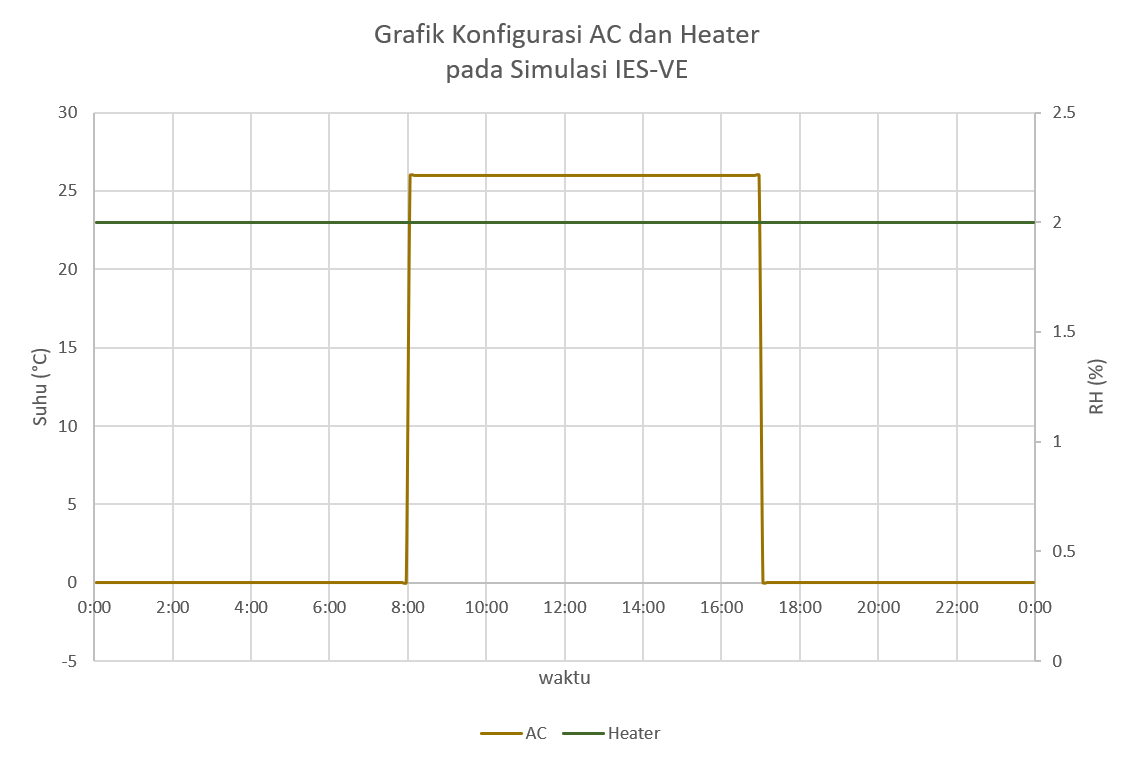
\includegraphics[width=0.4\textwidth]{figures/ACHTSimulasiIESVE}
			\caption{Data Konfigurasi AC dan \textit{Heater} pada Simulasi ISE-VE}
			\label{fig:4:ACHTSimulasiIESVE}
		\end{figure}
		
		\begin{figure}
			\centering
			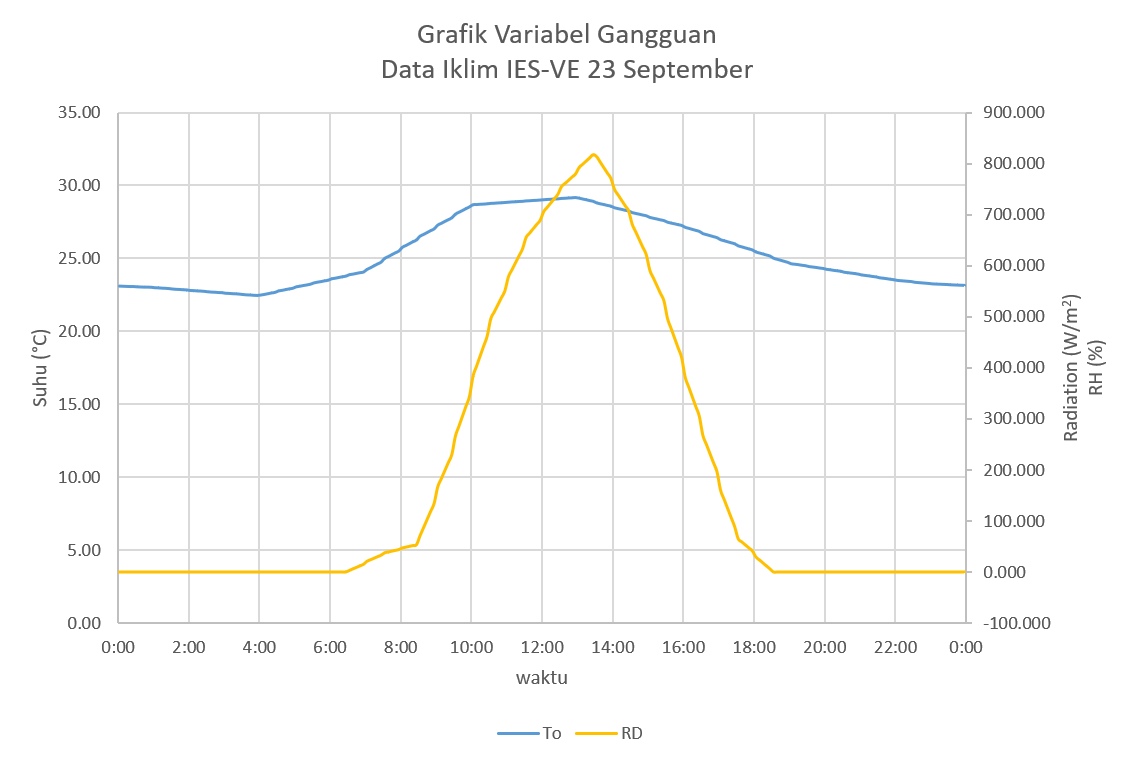
\includegraphics[width=0.4\textwidth]{figures/LoadSimulasiIESVE}
			\caption{Variabel Gangguan Simulasi ISE-VE}
			\label{fig:4:LoadSimulasiIESVE}
		\end{figure}
		
		\begin{figure}
			\centering
			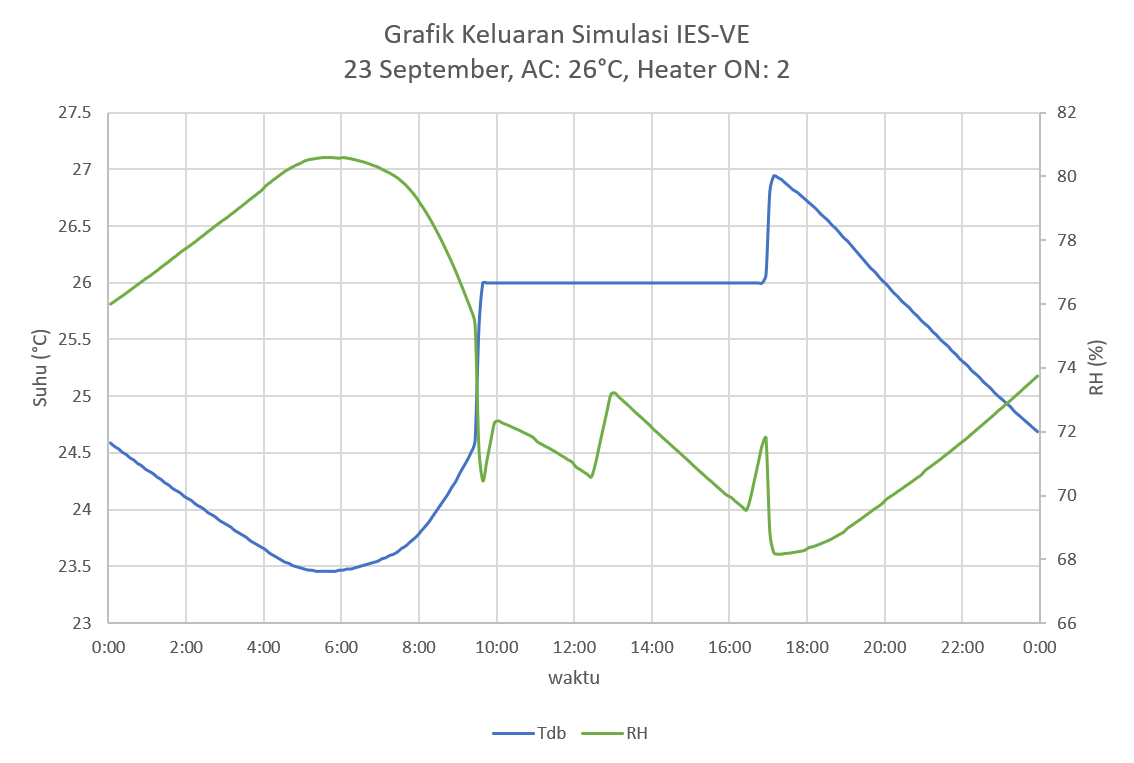
\includegraphics[width=0.4\textwidth]{figures/HasilSimulasiIESVE}
			\caption{Data Hasil Simulasi ISE-VE}
			\label{fig:4:HasilSimulasiIESVE}
		\end{figure}
		\vspace{2mm}
		
		\subsection{Identifikasi Sistem Pengendalian}
		
		Dalam perancangan sistem kendali, perlu diidentifikasi terlebih dahulu variabel-variabel yang terlibat pada suatu sistem. Terdapat beberapa variabel yang terlibat pada sistem \textit{climate chamber}. Variabel-variabel yang diangkat pada penelitian ini tunjukkan oleh diagram blok \textit{plant} pada Gambar \ref{fig:5:DiagramBlokPlant}. Berdasarkan diagram tersebut, dapat dikatakan bahwa sistem merupakan sistem MIMO (\textit{Multi Input Multi Output}) yaitu sistem yang memiliki beberapa masukan dan beberapa keluaran. Identifikasi sistem yang telah dilakukan akan menghasilkan suatu diagram blok fungsional sistem seperti yang ditunjukkan pada Gambar \ref{fig:5:DiagramBlokSistem}.\\
		
		\begin{figure}
			\centering
			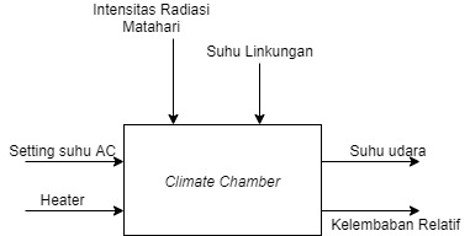
\includegraphics[width=0.35\textwidth]{figures/BlokDiagramPlant}
			\caption{Diagram Blok \textit{Plant}}
			\label{fig:5:DiagramBlokPlant}
		\end{figure}
		\vspace{1em}
		
		Dalam sistem \textit{climate chamber}, variabel manipulasi yang digunakan adalah \textit{setting} suhu AC dan \textit{heater} (jumlah \textit{heater} ON). Kemudian, variabel kontrol yang digunakan yaitu suhu udara (T$_{db}$) dan kelembapan relatif (RH) pada \textit{plant} (\textit{climate chamber}). Ada pula variabel gangguan sistem yaitu berupa intensitas radiasi matahari dan suhu lingkungan. Perubahan suhu oleh AC hanya mampu bekerja dengan kenaikan nilai sebesar 1$^\circ$C. Dengan memperhatikan \textit{manipulator} (\textit{final control elements}) yang digunakan, secara fisis RH tidaklah mungkin dapat dikendalikan oleh kontroler. Perubahan nilai RH yang terjadi diakibatkan oleh pengaruh AC secara tidak langsung. Untuk pengujian \textit{set point}, skenario pengujian mengadaptasi Tugas Akhir pengujian level sensasi termal yang dilakukan oleh Nadiya\cite{skripsiMuna}. Hanya saja pada penelitian menggunakan \textit{set point} step bertingkat dengan lompatan 2$^{\circ}$C dari nilai suhu sebesar 16$^{\circ}$C hingga 30$^{\circ}$C.\\
		
		\begin{figure}
			\centering
			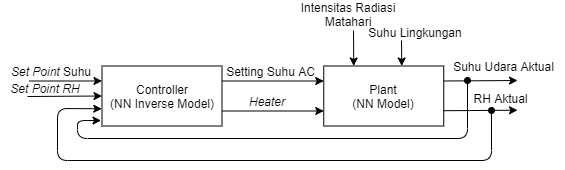
\includegraphics[width=0.5\textwidth]{figures/DiagramBlokFungsionalSistem}
			\caption{Diagram Blok Fungsional Sistem}
			\label{fig:5:DiagramBlokSistem}
		\end{figure}
		
		Kontroler pada \textit{climate chamber} memiliki enam buah variabel masukan dan dua buah variabel keluaran. Variabel masukan kendali ini yaitu nilai \textit{set point} suhu udara, \textit{set point} kelembapan relatif, nilai aktual umpan balik suhu udara, nilai aktual umpan balik kelembapan relatif, nilai umpan balik \textit{setting} suhu AC, dan nilai umpan balik \textit{heater}. Sementara, variabel keluaran kontroler ini adalah \textit{setting} suhu AC dan \textit{heater} (jumlah \textit{heater} ON).
		
		Untuk memaksimalkan kinerja kontroler, pada proses pelatihan JST (kontroler) dilakukan penskalaan terhadap semua variabel masukan JST menggunakan metode \textit{Min Max Scaling} kecuali variabel umpan balik \textit{setting} suhu AC dan variabel umpan balik \textit{heater}. Penskalaan bertujuan untuk meningkatkan kinerja JST menjadi optimal dengan menyamakan rentang nilai dan besar satuan dari setiap variabel (berupa rentang nilai dari 0 hingga 1). Masing-masing variabel diubah menjadi skala satuan dengan melakukan transformasi data secara statistik. Data dari setiap variabel akan dikurangi dengan nilai minimum variabel tersebut yang dikemudian dibagi oleh selisih dari nilai maksimum dan nilai minimum variabel tersebut. Dengan demikian, ditambahkan pula blok \textit{scaler} pada diagram blok sistem kontrol agar nilai masukan kontroler dapat disesuaikan.
		
		\begin{figure}
			\centering
			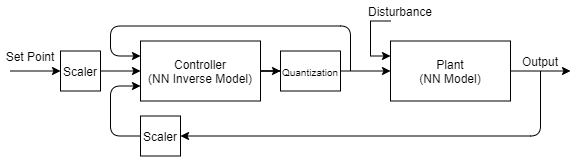
\includegraphics[width=0.5\textwidth]{figures/ControlDesignDiagramII}
			\caption{Diagram blok sistem kontrol berbasis JST}
			\label{fig:5:ConstrolSystemBlockDiagram}
		\end{figure}
		
		Diagram blok sistem kontrol juga memiliki blok tambahan berupa blok kuantisasi (\textit{Quantization}). Blok ini berperan sebagai penyesuai nilai variabel manipulasi yang dihasilkan kontroler. Hal ini dilakukan karena pada praktiknya nilai \textit{setting} suhu AC merupakan nilai bilangan bulat dan bukan nilai bilangan desimal. Hal ini pun berlaku untuk variabel manipulasi \textit{heater} di mana nilainya berupa nilai 0, 1, atau 2 yang menunjukkan jumlah \textit{heater} ON/menyala. Sehingga tidak mungkin ada nilai diantara nilai tersebut. Dengan demikian, diagram blok dipasangi sebuah blok kuantisasi (\textit{Quantization}) yang berfungsi untuk menghindari nilai desimal atau pun nilai yang berada di luar rentang nilai variabel manipulasi. Pada akhirnya dihasilkan diagram blok sistem kontrol yang ditunjukkan pada Gambar \ref{fig:5:ConstrolSystemBlockDiagram}.\\
		
		\subsection{Rancangan Kontroler JST}
		
		\subsubsection{Variasi Pembagiaan Data}
		
		Dalam memvariasikan pembagian data digunakan metode \textit{trial-and-error} berdasarkan artikel \cite{DataSplitting}. Pada penelitian ini, variasi pembagiaan data dilakukan dengan membandingkan beberapa variasi pembagiaan data ke dalam 5 variasi. Kemudian kinerja dari setiap pembagian data dibandingkan dengan konfigurasi \textit{hyperparameter} pada Tabel \ref{tbl:5:NeuronVariation}.
		
		\begin{table}
			\centering
			\caption{Tabel Daftar Variasi Pembagian Data}
			\label{tbl:5:NeuronVariation}
			\begin{tabularx}{\linewidth}{XX}\toprule
				\textbf{Pembagian Data} & \textbf{Persentase Data} \\ \toprule
				Pembagian Data 1 & (50\% 25\% 25\%) \\ \midrule
				Pembagian Data 2 & (60\% 20\% 20\%) \\ \midrule
				Pembagian Data 3 & (70\% 15\% 15\%) \\ \midrule
				Pembagian Data 4 & (80\% 10\% 10\%) \\ \midrule
				Pembagian Data 5 & (80\% 15\% 05\%) \\ \bottomrule
			\end{tabularx}
		\end{table}
		\vspace{1em}
		
		Model JST untuk membandingkan variasi pembagian data menggunakan arsitektur \textit{feedforward network} dengan 1 lapisan tersembunyi berisi 10 neuron. Pada tabel yang disajikan, pembagian data ditulis dengan format ’Pembagian Data n’ dan ’(x\% y\% z\%)’ dimana n = nomor variasi, x = pembagian data pelatihan, y = pembagian data validasi, dan z = pembagian data pengujian. Berdasarkan hasil variasi yang ditunjukkan pada Gambar \ref{fig:5:DataSplittingVariation}, didapatkan pembagian data terbaik yaitu pembagian data bernama "Pembagian Data 4". Data dibagi menjadi 3 bagian, yakni 80\% data pelatihan, 10\% data validasi, dan 10\% data pengujian.\\
		
		\begin{figure}
			\centering
			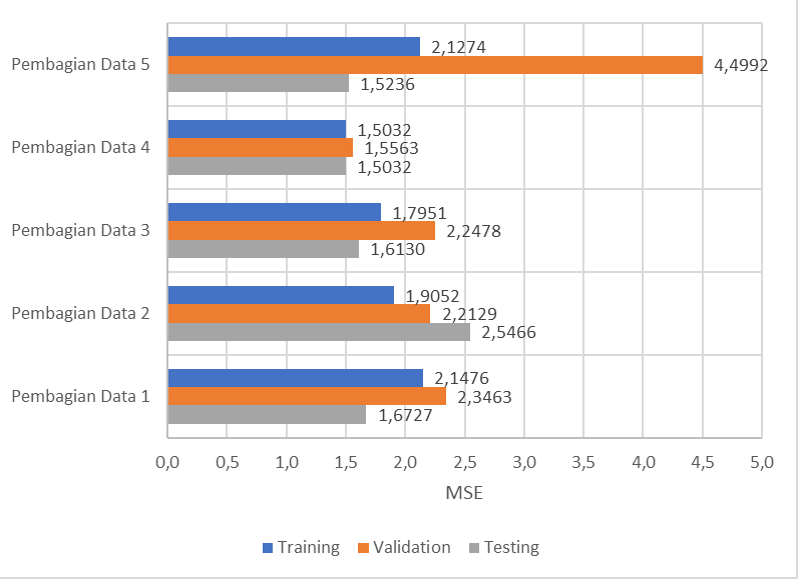
\includegraphics[width=0.5\textwidth]{figures/VariasiPembagianDataJSTKontroler}
			\caption{Grafik Variasi Pembagian Data}
			\label{fig:5:DataSplittingVariation}
		\end{figure}
		
		\subsubsection{Variasi Arsitektur JST Kontroler}
		
		Pada perancangan model JST kontroler digunakan 2 variasi fungsi aktivasi, yaitu fungsi tansig (fungsi \textit{hyperbolic tanget}) dan fungsi logsig (fungsi sigmoid). Kemudian masing-masing dilatih dengan jumlah neuron yang bervariasi dari 5 neuron hingga 60 neuron dengan lompatan sebesar 5 neuron. Dari proses variasi ini, didapatkan hasil bahwa model yang menggunakan fungsi aktivasi tansig dengan 35 neuron menghasilkan kinerja dengan nilai MSE terkecil. Hasil dari variasi ini ditunjukkan pada Gambar \ref{fig:5:ActivationVariation}.
		
		\begin{figure}
			\centering
			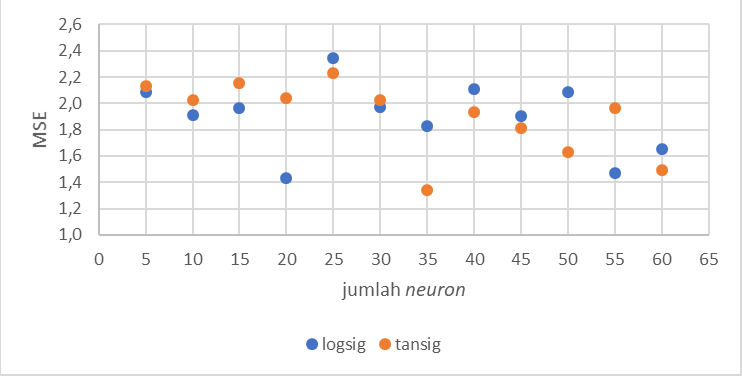
\includegraphics[width=0.5\textwidth]{figures/ActivationVariation}
			\caption{Grafik Persebaran MSE Variasi Arsitektur JST Kontroler}
			\label{fig:5:ActivationVariation}
		\end{figure}
		
		\begin{figure}
			\centering
			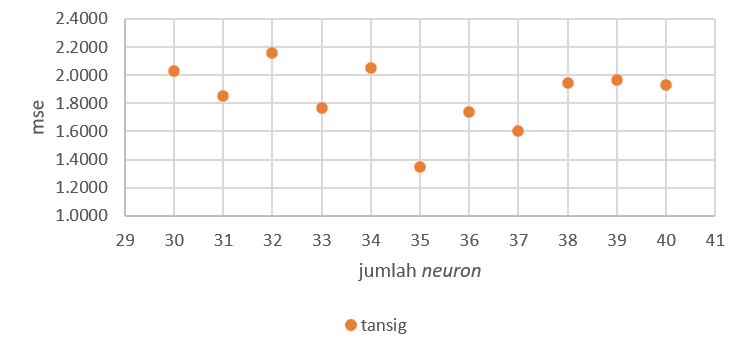
\includegraphics[width=0.5\textwidth]{figures/NeuronVariation}
			\caption{Grafik Persebaran MSE Variasi Arsitektur JST Kontroler}
			\label{fig:5:NeuronVariation}
		\end{figure}
		\vspace{1em}
		
		Kemudian arsitektur JST divariasikan kembali menggunakan fungsi aktivasi tansig dari 30 neuron hingga 40 neuron dengan lompatan sebesar 1 neuron untuk mengetahui kinerja model pada jumlah neuron yang berdekatan. Setelah dilakukan variasi, didapatkan hasil bahwa model JST dengan 35 neuron masih merupakan model arsitektur terbaik dengan nilai MSE terkecil. Hasil variasi ini dapat dilihat pada Gambar \ref{fig:5:NeuronVariation}.
		
		\subsubsection{Hasil Rancangan Model JST Kontroler}
		Setelah dilakukan perancangan model JST melalui variasi arsitektur model, didapatkan rancangan model JST kontroler terbaik. Model JST dibangun dengan arsitektur \textit{feedforward neural network} 1 lapisan tersembunyi dengan 35 neuron. Model JST menggunakan fungsi aktivasi tansig (\textit{hyperbolic tanget}) dan algoritma pembelajaran Levenberg-Marquardt. Model JST Kontroler terbaik memiliki nilai \textit{hyperparameter} yang diringkas pada Tabel \ref{tbl:5:NNControl}.
		
		\begin{table}
			\centering
			\caption{Tabel Rancangan Kontroler JST (\textit{NN Inverse Model})}
			\label{tbl:5:NNControl}
			% use packages: array
			\begin{tabularx}{\linewidth}{XX}\toprule
				\textbf{Nama Hyperparameter} & \textbf{Nilai Hyperparameter} \\ \toprule
				Arsitektur & Feedforward Neural Network \\ \midrule
				Pembagian Data & 80\% 10\% 10\% \\ \midrule 
				Jumlah Layar Tersembunyi & 1 \\ \midrule
				Jumlah Neuron pada Layar & [35] \\ \midrule
				Fungsi Aktivasi Layar & Hyperbolic Tangent (tansig) \\ \midrule
				Algoritma Pembelajaran & Levenberg-Marquardt \\ \midrule
				Mean Absolute Error (MAE) & AC: 0,37$^\circ$C ; HT: 0,02\\ \midrule
				Mean Squared Error (MSE) & AC: 2,68$^\circ$C ; HT: 0,01\\ \midrule
				Koefisien Korelasi (R) & AC: 99,12\% ; HT: 99,65\% \\ \bottomrule
			\end{tabularx}
		\end{table}
	
		\vspace{2mm}
				
		\subsection{Hasil Simulasi Kontrol SIMULINK}
		
		Pada simulasi kontrol, digunakan nilai \textit{set point} sesuai dengan uji eksperimental level sensasi termal yang dilakukan oleh Nur Muna pada \textit{climate chamber}\cite{skripsiMuna}. Perbedaannya, pada penelitian ini variasi naik turun suhu dari 16$^\circ$C hingga 30$^\circ$C menggunakan lompatan sebesar 2$^\circ$C.
		
		\subsubsection{Skenario Pemanasan Pendinginan dengan Variabel Gangguan Konstan}
		
		Pada simulasi ini digunakan nilai variabel gangguan konstan sebesar 26,8$^\circ$C untuk suhu lingkungan dan 423,343 $W/m^2$ untuk intensitas radiasi matahari. Nilai-nilai variabel gangguan tersebut merupakan nilai rerata dari variabel gangguan pada jam operasi penggunaan \textit{climate chamber}, yaitu pukul 08:00 WIB sampai dengan pukul 17:00 WIB. Berdasarkan hasil simulasi, kontroler mampu mengendalikan suhu ruang dan kelembapan relatif mengikuti nilai \textit{set point}. Akan tetapi, kontroler tidak mampu menaikan suhu ruang mencapai nilai lebih dari 27$^\circ$C. Hal ini dapat terjadi diakibatkan nilai manipulator AC tidak mampu melebihi nilai maksimum (SET 30$^\circ$C). Kombinasi \textit{set point} dan hasil simulasi ditunjukkan pada Gambar \ref{fig:5:SimulinkTd} untuk suhu ruang dan Gambar \ref{fig:5:SimulinkRH} untuk kelembapan relatif.
		
		Dengan meninjau nilai variabel manipulasi AC yang ditunjukkan pada Gambar \ref{fig:5:SimulinkAC}, dapat dilihat bahwa untuk mengendalikan suhu mencapai \textit{set point} 26$^\circ$C, perangkat AC perlu mengeluarkan sinyal sebesar 28$^\circ$C (waktu ke-100 hingga ke-120). Dengan demikian, ketika \textit{set point} bernilai 28$^\circ$C, perangkat AC hanya mampu mengeluarkan sinyal maksimum 30$^\circ$C (waktu ke-120 hingga ke-140).
		
		\begin{figure}
			\centering
			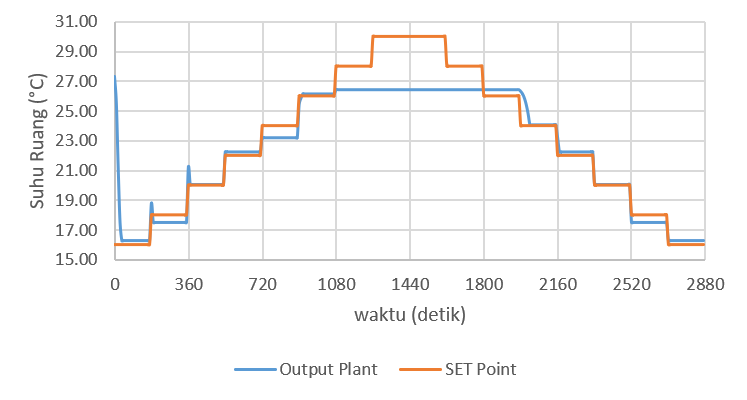
\includegraphics[width=0.5\textwidth]{figures/Simulink1Td}
			\caption{Grafik Hasil Simulasi Simulink untuk Suhu Ruang}
			\label{fig:5:SimulinkTd}
		\end{figure}
		\vspace{1em}
		
		\begin{figure}
			\centering
			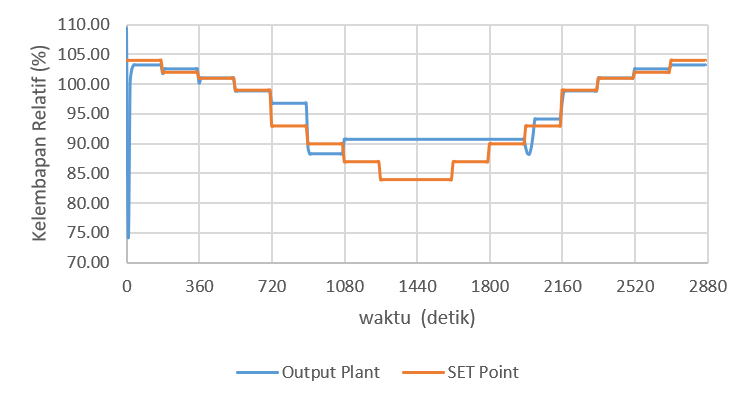
\includegraphics[width=0.5\textwidth]{figures/Simulink1RH}
			\caption{Grafik Hasil Simulasi Simulink untuk Kelembapan Relatif}
			\label{fig:5:SimulinkRH}
		\end{figure}
		\vspace{1em}
		
		\begin{figure}
			\centering
			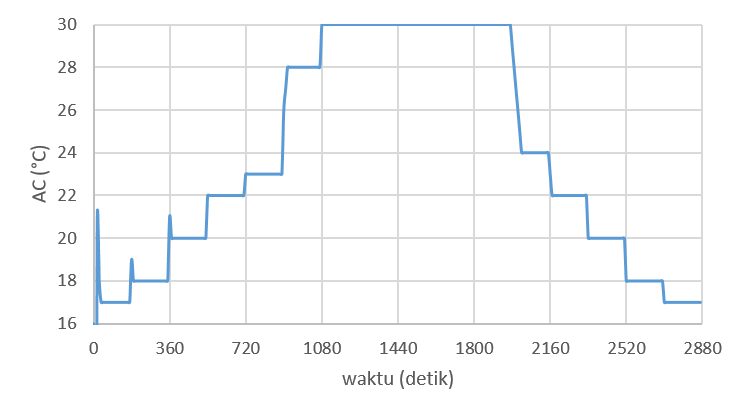
\includegraphics[width=0.5\textwidth]{figures/Simulink1AC}
			\caption{Grafik Variabel Manipulasi AC pada Simulasi Simulink}
			\label{fig:5:SimulinkAC}
		\end{figure}
		\vspace{1em}
		
		\begin{figure}
			\centering
			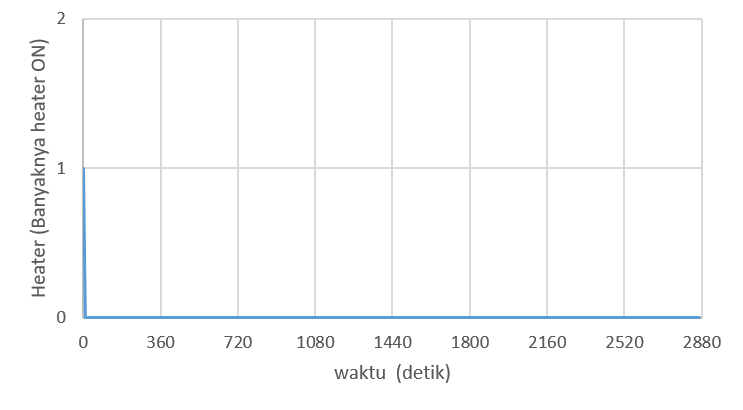
\includegraphics[width=0.5\textwidth]{figures/Simulink1HT}
			\caption{Grafik Variabel Manipulasi \textit{Heater} pada Simulasi Simulink}
			\label{fig:5:SimulinkHT}
		\end{figure}
		\vspace{1em}
		
		Kurangnya kehandalan kinerja kontroler pada penelitian ini untuk mengendalikan suhu ruang di atas \textit{set point} 26$^\circ$C disebabkan oleh salah satu kelemahan model JST dalam pemodelan \textit{plant}. Secara fisis, proses pemanasan pada sistem bangunan (dalam hal ini \textit{climate chamber}) membutuhkan waktu yang cukup lama. Dengan demikian, proses pemanasan pada kenyataannya tetap bisa mencapai \textit{set point} suhu di atas 26$^\circ$C. Hanya saja proses tersebut membutuhkan waktu (\textit{settling time}) yang cukup lama. Akan tetapi, proses tersebut tidak dapat disimulasikan secara sempurna pada penelitian ini dikarenakan model JST \textit{plant} yang dibangun oleh Tri Hartanto\cite{skripsiTanto} hanya berupa model pasangan data dan bukan berupa model yang bergantung terhadap waktu. Sehingga, model JST \textit{plant} hanya dapat langsung mengeluarkan suatu nilai keluaran setiap menerima nilai masukan.
		
		Ditinjau dari \textit{set point} 16$^\circ$C hingga 26$^\circ$C, didapatkan nilai \textit{steady-state error} untuk suhu ruang sebesar 0,15$^\circ$C pada proses pemanasan dan sebesar 0,2$^\circ$C pada proses pendinginan. Lalu, didapatkan pula nilai \textit{steady-state error} untuk kelembapan relatif sebesar 0,05\% pada proses pemanasan dan sebesar 0,02\% pada proses pendinginan. Sehingga rerata nilai \textit{steady-state error} sebesar 0,18$^\circ$C untuk suhu ruang dan sebesar 0,04\% untuk kelembapan relatif.
		
		\subsubsection{Skenario Pemanasan Pendinginan dengan Variabel Gangguan Bergerak}
		
		Pada skenario ini digunakan data variabel gangguan pada 21 Juni 2019 yang bergerak dari pukul 08:03 sampai dengan 08:51 WIB. Nilai dari variabel gangguan ditunjukkan pada Gambar \ref{fig:5:Simulink2To} untuk suhu lingkungan dan \ref{fig:5:Simulink2RD} untuk intensitas radiasi matahari. Pada skenario ini, nilai \textit{set point} yang digunakan senilai dengan nilai \textit{set point} pada simulasi dengan variabel gangguan konstan.
		
		Hasil simulasi dengan variabel gangguan bergerak pun menunjukan kinerja yang kurang optimal. Berdasarkan Gambar \ref{fig:5:Simulink2Td}, dapat dilihat bahwa kontroler tidak mampu menaikan suhu ruang mencapai nilai lebih dari 27$^\circ$C. Dapat dilihat pula bahwa terjai lonjakan nilai suhu udara pada detik ke-1980. Lonjakan tersebut terjadi akibat penonaktifan AC yang dilakukan oleh kontroler yang dapat dilihat pada Gambar \ref{fig:5:Simulink2AC}. Pada proses pendinginan, nilai \textit{steady-state error} tampak lebih besar dibandingkan saat proses pemanasan. Hal ini mungkin disebabkan karena kenaikan suhu lingkungan dan intensitas radiasi matahari. Walaupun nilai galat membesar, dapat dilihat bahwa pada proses pendinginan kontroler tetap berupaya untuk mengikuti perubahan \textit{set point}.\\
		
		\begin{figure}
			\centering
			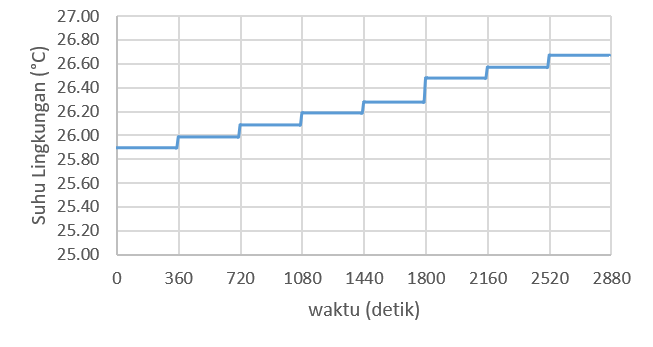
\includegraphics[width=0.5\textwidth]{figures/Simulink2To}
			\caption{Grafik Nilai Variabel Gangguan Suhu Lingkungan}
			\label{fig:5:Simulink2To}
		\end{figure}
		
		\begin{figure}
			\centering
			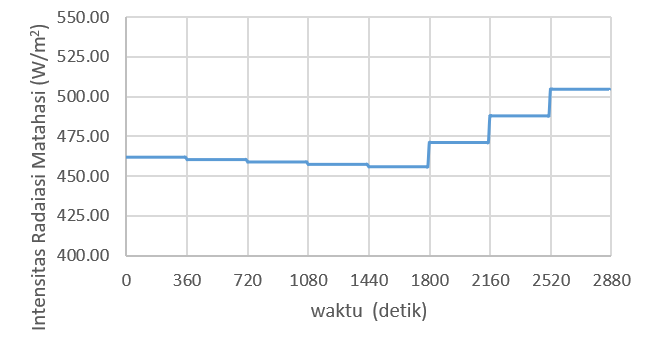
\includegraphics[width=0.5\textwidth]{figures/Simulink2RD}
			\caption{Grafik Nilai Variabel Gangguan Intensitas Radiasi Matahari}
			\label{fig:5:Simulink2RD}
		\end{figure}
		\vspace{1em}
		
		\begin{figure}
			\centering
			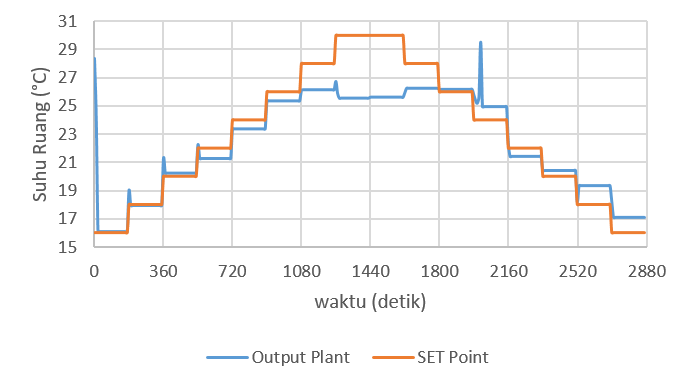
\includegraphics[width=0.5\textwidth]{figures/Simulink2Td}
			\caption{Grafik Hasil Simulasi Simulink untuk Suhu Ruang}
			\label{fig:5:Simulink2Td}
		\end{figure}
		\vspace{1em}
		
		\begin{figure}
			\centering
			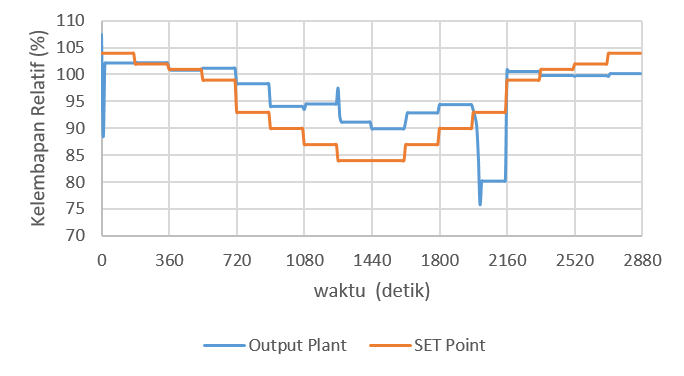
\includegraphics[width=0.5\textwidth]{figures/Simulink2RH}
			\caption{Grafik Hasil Simulasi Simulink untuk Kelembapan Relatif}
			\label{fig:5:Simulink2RH}
		\end{figure}
		\vspace{1em}
		
		\begin{figure}
			\centering
			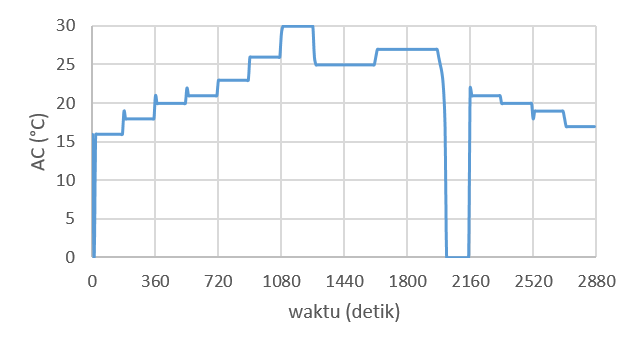
\includegraphics[width=0.5\textwidth]{figures/Simulink2AC}
			\caption{Grafik Variabel Manipulasi AC pada Simulasi Simulink}
			\label{fig:5:Simulink2AC}
		\end{figure}
		\vspace{1em}
		
		\begin{figure}
			\centering
			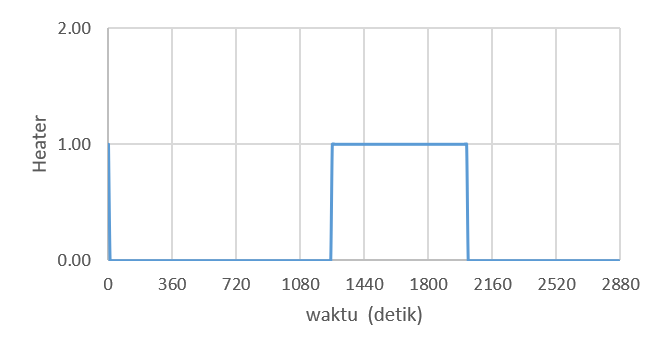
\includegraphics[width=0.5\textwidth]{figures/Simulink2HT}
			\caption{Grafik Variabel Manipulasi \textit{Heater} pada Simulasi Simulink}
			\label{fig:5:Simulink2HT}
		\end{figure}
		\vspace{1em}
		
		\subsection{Analisis Kegagalan Kendali}
		
		Dari hasil 2 simulasi yang telah dijabarkan, kontroler jarang sekali mengaktifkan 2 \textit{heater} bahkan disaat ingin mencapai suhu yang tinggi. Hal ini menimbulkan kecurigaan terhadap rentang kinerja JST, baik pada model kontroler maupun model \textit{plant}. Untuk mengetahui penyebab kegagalan, dilakukan kembali simulasi dimana kontroler berhasil mengaktifkan 2 perangkat \textit{heater}. Simulasi ini dilakukan dengan nilai variabel gangguan sebesar 27$^\circ$C untuk suhu lingkungan dan sebesar 600 $W/m^2$ untuk intensitas radiasi matahari.
		
		Berdasarkan hasil simulasi tersebut, dapat disimpulkan bahwa kegagalan pengendalian bukanlah disebabkan oleh tidak aktifnya 2 buah perangkat \textit{heater}. Selanjutnya, dicoba untuk dianalis model \textit{plant} yang dibangun oleh Hartanto. Pengujian dilakuakan dengan nilai variabel gangguan yang sama dan nilai AC 30$^\circ$C serta 2 \textit{heater} ON.
		
		Berdasarkan analisis, diketahui bahwa \textit{plant} memang tidak mampu untuk menghasilkan keluaran suhu diatas 28$^\circ$C. Dengan begitu, perlu ditelaah kembali mengenai data yang digunakan. Setelah diteliti, kurangnya keandalan kontroler ternyata disebabkan oleh data simulasi yang dinilai kurang cukup mewakili kondisi lingkungan termal di suhu yang tinggi. Hal ini disebabkan karena tidak dilakukannya validasi di suhu tinggi pada penelitian Kurniawan \cite{skripsiIchfan}. Dengan demikian, model yang telah dibangun Hartanto pun pada akhirnya tidak mampu menghasilkan skenario dimana lingkungan termal \textit{climate chamber} mencapai suhu diatas 28$^\circ$C.\\
		
		\section{Kesimpulan}
		Rancangan kontroler berbasis jaringan saraf tiruan memiliki nilai \textit{steady-state error} sebesar 0,18$^\circ$C untuk suhu ruang. Kontroler berbasis jaringan saraf tiruan yang dihasilkan dibangun dengan pembagian data 80\% data latih, 10\% data validasi, dan 10\% data uji. Model Kontroler JST menggunakan fungsi aktivasi \textit{hyperbolic tangent} dengan algoritma pembelajaran Levenberg-Marquardt. Model Kontroler JST terdiri dari 1 lapisan tersembunyi dengan 35 neuron. Akan tetapi, kontroler tidak mampu mengendalikan suhu ruang \textit{climate chamber} di atas nilai \textit{set point} 26$^\circ$C dikarenakan data lingkungan termal dari Model IES-VE kurang mewakili kondisi sistem pada suhu yang tinggi.\\
		
		\section{Saran}
		\begin{enumerate}
			\item Disarankan untuk melakukan validasi model di nilai suhu yang tinggi terlebih dahulu apabila menggunaan model IES-VE yang serupa.
			\item Memperkaya data pelatihan model JST menggunakan data pengukuran langsung pada \textit{climate chamber} dalam merancang kontroler JST.
			\item Menambahkan semacam \textit{manipulator}/aktuator pada \textit{climate chamber} untuk memanipulasi kelembapan relatif ruang secara langsung seperti penelitian yang dilakukan oleh Moon \cite{paper22JJkim}. Contoh: \textit{humidifier} dan \textit{dehumidifier}.
			\item Menambahkan variabel kontrol lainnya ke dalam rancangan kontroler, seperti kecepatan angin, suhu radian, RH lingkungan, dsb.
		\end{enumerate}
		\vspace{2mm}
		
		\section*{Ucapan Terima Kasih}
		Penulis mengucapkan banyak terima kasih kepada kedua pembimbing tugas akhir penulis, yaitu Faridah, S.T., M.Sc., dan Ir. Agus Arif, M.T., Tim \textit{Climate Chamber} DTNTF, serta rekan-rekan perkuliahan UGM: M. N. Fathurrahman, Irfanda Husni Sahid, M. Armand A., Tri Hartanto, Ivan Ega Pratama, dan Vandy Achmad.
		
		\bibliographystyle{skripsi}
		\bibliography{pustaka}
	\end{body}
\end{document}